\chapter{Monte Carlo (MC) Samples}
\label{sec:MCSamples}

In order to analyze the data we use the computer-generated so-called pseudo-data samples using the software that simulates the physical processes that happen in the detector. This pseudo-data is also called "Monte Carlo" or MC and its purpose is to construct the data samples based on the theoretical predictions of our physical model. Ideally, the MC samples should be as close to the real data as possible, allowing us to inspect all the stages of the analysis with a great precision. MC is used for tuning of the reconstruction algorithms (see Sec.~\ref{sec:Reconstruction}), calibration of the calorimeter (see Sec.~\ref{sec:Calibration}), calculation of the efficiencies (see Sec.~\ref{sec:Efficiency}), estimation of the background (see Sec.~\ref{sec:Bkg}), and finally for the comparison of the data to the theoretical predictions (see Sec.~\ref{sec:Results}). Unfortunately, we are unable to recreate the data samples precisely, so some corrections are made by the means of reweightings (see Sec.~\ref{sec:MC_correction}).

\begin{figure}
\center{
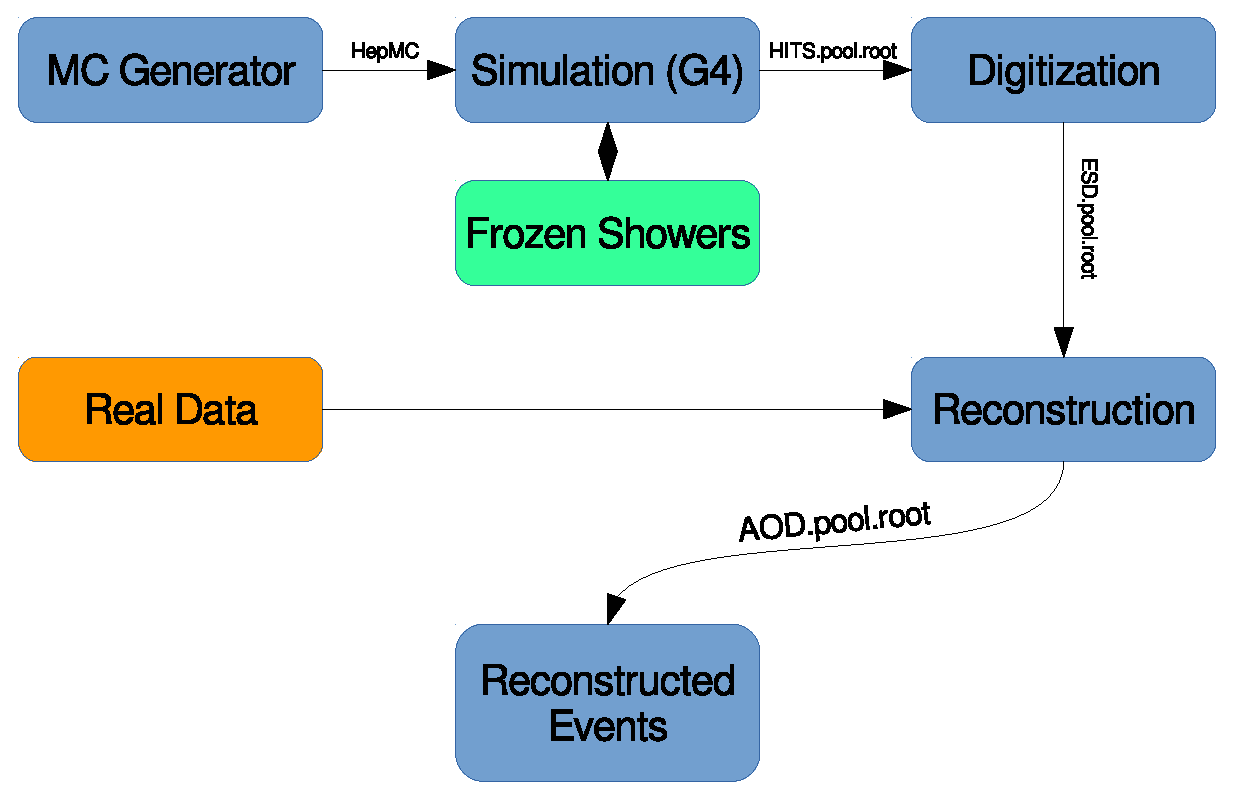
\includegraphics[width=0.7\textwidth]{figures/MC_production_chain.eps}
\caption{Diagram of the ATLAS MC production chain}
\label{fig:MC_gen}}
\end{figure}

The process of generating of the MC samples consists of several stages, which can be seen in the diagram of the MC production chain in Fig.~\ref{fig:MC_gen}. Here are the short descriptions of every step of the production:
\begin{enumerate}
\item The simulation of the $pp$ collision, which involves the production and the decay of high-energy particles (done by the MC generators, see sec.~\ref{sec:MC_gen}).
\item The simulation of interactions between the high-energy particles and the substance of the detector (done by the Geant4 software~\cite{lib:geant4}, see sec.~\ref{sec:MC_sim}).
\item The simulation of the detector response based on the amount of deposited energy in different parts of the detectors (done by the ATLAS software).
\item The reconstruction process runs the same way as for the genuine data samples, it is fully described in Chapter~\ref{sec:Reconstruction}.
\end{enumerate}
The simulation process takes a lot of time, with the most time-consuming process being the simulation of the particles passing through the detector, or even more precise, through the EM-calorimeters, as the calorimeters consist of the very dense materials (e.g. lead and liquid argon) and hence the incoming high-energy particles produce the large showers with the tens of thousands of lower-energy particles. There are several technics used to speed up the process, but most of them produce the different result from the standard not-optimized simulation, which makes them unusable for many types of analysis (including \Zee). The only technology which gives the result close enough to the standard simulation to be enabled for all analysis samples by default is the Frozen Showers, which will be fully described in sec.~\ref{sec:MC_FS}. In the following sections the details of the steps involved in the MC production chain are discussed. In sec.~\ref{sec:MC_gen} the details of the various MC generators (first step) are given, and in sec.~\ref{sec:MC_sim} the rest of the production chain is discussed, with the focus on the simulation of the passage of the high-energy particles through the detector (second stage) and the digitization process (third stage). The reconstruction process is discussed fully in sec.~\ref{sec:Reconstruction}.

\section{MC generators used in ATLAS experiment}
\label{sec:MC_gen}

The first stage of the MC production is the simulation of the $pp$ collision itself. The simulation of this process is based on the standard model, and tries to account for every significant aspect of it. The core of the simulation is the calculation of the matrix element (ME) of the $pp$ interaction, which can be done in different orders. The simplest case is the leading order (LO), which in case of the $\Zee$ is the bare Drell-Yan diagram, with no loops or extra legs. The simulations in the leading order are not precise, and generally the next to leading order (NLO) or next to next to leading order (NNLO) are used instead, with one or two extra loops/legs respectively. The calculation of the matrix element in higher orders is very complex, and in order to increase the precision of the simulation the additional particles are simulated outside of the ME. Additional QCD particles are generated using the "parton shower" (PS) technique, which is to simulate the QCD radiation on every parton independently, using the formulas not unlike the ME. The PS technique is widely adopted and used in every MC generator. Additional QED radiation is generated in a similar way by the independent package named "Photos"~\cite{lib:photos}, with the similar technique. This package can be used in conjunction with other MC generators.

Here is the list of the most noticeable MC generators used in ATLAS analyses:
\begin{itemize}
\item \Herwig~\cite{lib:MC_herwig} is a general-purpose event generator for high-energy processes, with particular emphasis on the detailed simulation of QCD parton showers. The program provides a full simulation of hard lepton-lepton, lepton-hadron and hadron-hadron scattering and soft hadron-hadron collisions in a single package, and has the following special features:
\begin{itemize}
\item Initial- and final-state QCD jet evolution with soft gluon in terference taken into account via angular ordering.
\item Color coherence of (initial and final) partons in all hard subprocesses, including the production and decay of heavy quarks and supersymmetric particles.
\item Azimuthal correlations within and between jets due to gluon interference and polarization.
\item A cluster model for jet hadronization based on non-perturbative gluon splitting, and a similar cluster model for soft and underlying hadronic events.
\item A space-time picture of event development, from parton showers to hadronic decays, with an optional color rearrangement model based on space-time structure.
\end{itemize}
In MC11c \Herwig\ is used to provide the parton showering for other generators.

\item \Pythia~\cite{lib:MC_pythia6} (and an updated version \Pythiaeight~\cite{lib:MC_pythia8}) is a generator with the objective to provide as accurate as possible a representation of event properties in a wide range of reactions, within and beyond the Standard Model, with emphasis on those where strong interactions play a role, directly or indirectly, and therefore multihadronic final states are produced. The physics is then not understood well enough to give an exact description, instead the program has to be based on a combination of analytical results and various QCD-based models.

\item \Powheg~\cite{lib:MC_powheg} is a hard event generator for heavy quark production in hadronic collisions. It is accurate at the next-to-leading order in QCD, and it can be interfaced to Shower Monte Carlo programs like \Herwig\ and \Pythia, in such a way that both the leading logarithmic accuracy of the shower and the NLO accuracy are maintained in the output. This generator is the main MC generator used in 2011 analyses.

\item \Mcatnlo~\cite{lib:MC_mcatnlo} is a practical implementation, based upon the Fortran \Herwig\ and \Herwigpp\ event generators, of the \Mcatnlo\ formalism, which allows one to incorporate NLO QCD matrix elements consistently into a parton shower framework.

\item \Sherpa~\cite{lib:MC_sherpa1, lib:MC_sherpa2} is a multi-purpose tool which contains a very flexible tree-level matrix-element generator for the calculation of hard scattering processes within the Standard Model and various new physics models.  The emission of additional QCD partons off  the  initial  and  final  states  is  described through a parton-shower model without the need of an additional generator. This generator is only used for the signal MC.
\end{itemize}

\subsection{Signal MC}

The part of Monte Carlo simulation which represents \Zee\ events is called "signal MC". \tbu uses
As well as the standard model itself, the MC generators have parameters which can't be theoretically predicted, and should be found empirically. This process is called "MC tuning", and is done separately for every experiment, because the tune which will describe well one experiment won't fit for other. The tunes used in ATLAS are described in~\cite{lib:MC_tune1, lib:MC_tune2}.

The other important part of MC customization is the PDF set. PDF stands for "parton distribution function". It is a model that describes the energy distribution between quarks inside the proton. There are several PDF sets calculated based on the data from different experiments. The sets are distributed with the LHAPDF software~\cite{lib:lhapdf}, which represents the full compendium of PDF sets calculated and validated by this time. The biggest contributions to the PDF collection were done by the Tevatron and HERA experiments. The PDF sets used in the current analyses are dicribed in~\cite{lib:MC_pdfct10, lib:MC_pdfcteq6l1}.

\subsection{Background MC}

The part of Monte Carlo simulation which represents different processes which can be misinterpreted as \Zee\ is called "background MC". There are several background processes that can be simulated using MC, and most of them (all but one) are electroweak processes, that is why the background MC is also called an "electroweak background" as opposed by the "multi-jet background" or also "QCD background" which is the background from the multi-jet hadronic processes, which cannot be reliably simulated.

We use seven different types of backgrond MCs.
\begin{itemize}
\item \Wenu, the decay of $W$ boson into electron and neutrino. Can be misinterpreted as $Z$ decay if another electron is reconstructed in the same event, most notably, when a jet is misinterpreted as an electron (a "fake electron").
\item \Wtau, the decay of $W$ boson into tau and neutrino. Can be misinterpreted if tau decays into electron, and another unrelated electron is reconstructed as in the previous case.
\item \Ztau, the decay of $Z$ boson into two taus. Can be misinterpreted if at least one tau decays into electron, and another electron is reconstructed. The case of both tau decaying into electrons and $Z$ boson constructed from them is is also possible, since the mass window is wide enough for that.
\item \ttbar\ events, which have lots of decay modes, and thus can be misinterpreted as almost anything, including \Zee. The most common case is \ttbar\ decaying into $W^{+}W^{-}\antibar{b}$, and thus falling into the $WW$ category.
\item $WW$, can be misinterpreted if both bosons decay into $e\nu$.
\item $WZ$, and $ZZ$ events. In our analysis we filter such events, and thus misinterpretation of e.g. $WZ$ event as \Zee\ event is a background event for us.
\end{itemize}

\section{MC simulation process in ATLAS}
\label{sec:MC_sim}

Although the whole process of the production of the MC samples can be considered as "simulation", in this context "the simulation process" refers to the particular stage of the whole production chain: the simulation of the propagation of the high-energy particles through the matter of the detector. It is done using the Geant4 software and the highly-accurate 3D model of the detector. The simulation in Geant4 is done as a discrete step-by-step process, with the length of the step being calculated dynamically for each particle, based on particle energy and the physical processes that happen to that particle. Because of that the simulation of the particles in vacuum takes much less time than in heavy matter. That is the reason why the majority of the simulation time is spent in calorimeters: they are built of the densest material there is in explicit purpose to stop as many particles as possible.

The output of the simulation stage is "hits", the 4D vertexes of energy deposits in sensitive areas of the detectors. The next stage is to simulate the work of the detector itself, or to convert the energy deposits into detector response, which are usually voltages on the read-out channels. This process is called "digitization", because its output is "digits" which the read-out channels provide. During this stage all features of the detector logic are simulated (e.g. electric noises or channel-dependent variations). This is done by the internal ATLAS digitization software, and because it requires an intimate knowledge of every particular sub-detector, parts of it are maintained by separate groups related to the respective sub-detectors.

The last step in the production chain is the same for both MC and genuine data samples, as the digitization process aims to provide the same data as we get from the detector during production runs. During this step the responses from the detector are reconstructed into physical objects, which is done in two steps. First step is more on the technical side, during which the response from the trackers is reconstructed into tracks and the response from the calorimeters is reconstructed into clusters. The second stage is physical and depends on the analysis. During this stage the tracks and clusters are combined into the physical particles. The flavors of this stage of reconstruction include e/gamma, jet/EtMiss/tau, b tagging and muon. $\Zee$ analysis uses the first: e/gamma flavored reconstruction. This process is done using the internal ATLAS reconstruction software. More on the reconstruction process with respect to the real data from the detector is in Sec.~\ref{sec:Reconstruction}.

The result of the reconstruction is the data stored in the special format called AOD (Analysis Data Object), which is also developed internally by ATLAS. AODs can be read by the ATLAS analysis framework, which gives easy access to all reconstructed objects.

\subsection{Frozen Showers}
\label{sec:MC_FS}
The frozen showers system (FS) is a system that is designed to speed up the geant4 simulation process inside the EM calorimeters. The main principle of FS is to substitute the low-energy particles with the EM-showers, which are pre-simulated and stored in the libraries (see Fig.~\ref{fig:MC_FS_method}). These libraries must be generated in advance for each calorimeter and for each type of particles which is needed to be fast-simulated during the production simulation. The generation process consists mostly of the simulating of the low-energy particles and saving the information about every energy deposition this particle made. The array of these deposits or "hits" passes through several post-processing procedures in order to reduce its size, and becomes a "shower".

\begin{figure}
\center{
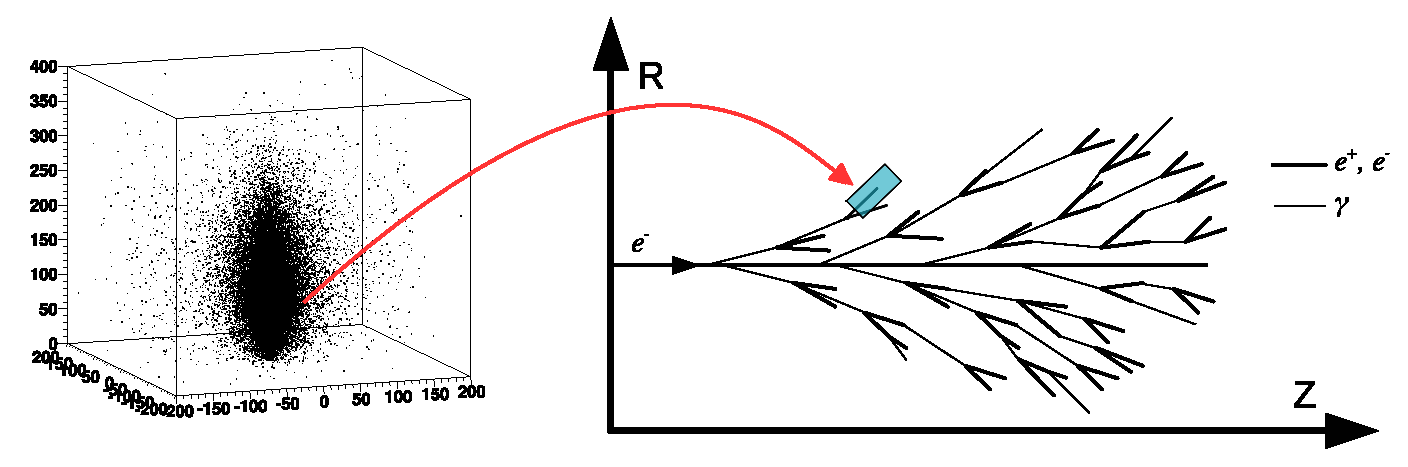
\includegraphics[width=1.0\textwidth]{figures/MC_FS_method.eps}
\caption{Diagram showing the shower substitution of the low-energy particle, during the high-energy particle simulation.}
\label{fig:MC_FS_method}}
\end{figure}

The generation of the shower library is thus a preparatory procedure, which needs to be done every time when something is changed in the geant4 simulation process. The examples are the change of the geant4 version used, or the change in the detector geometry. Usually these changes applied between the MC campaigns, which means that the new set of libraries needs to be generated for each campaign. In order to improve results of FS-enabled simulation the libraries are then tuned: the shape and the energy response of the stored showers are slightly changed to provide the needed changes in the resulting simulation.

The processes of the library generation (and tuning) and the production use FS system would be described separately in the two following sections.

\subsubsection{FS library generation}
\label{sec:MC_FS_gen}

The library is the set of the showers simulated from the low-energy particles of the same (needed) type. The library should be able to provide the shower for any particle of this type within the determent energy bounds and inside the corresponding sub-detector. Thus, the showers populating the library should also be generated with all the possible energies and in all of the sub-detectors volume. To do this we need to generate the low-energy particles (as during the generation stage described in sec.~\ref{sec:MC_gen}) with different energies and different vertexes that covers continuously both volume and energy range.

The easiest way to do it is to use a particles gun: a tool that can create a particle with arbitrary type, momentum and vertex. This way we will get a library uniformly populated by libraries in every part of its kinematic space. This approach has two major disadvantages. First, it reduces the quality of the simulation. As we can't match all of the particle parameters while searching for the suitable shower within the library (it will take too much time time and require the libraries of enormous sizes), we disregard some of them and introduce large bins on some others. Because of that the matched shower can have substantially different properties then the required particle. The second problem is the oversized library. During the production simulations the libraries from some part of the kinematic space (e.g. with the lowest energy of $0-10 MeV$ as opposed to $500-1000 MeV$) are requested more often than others. This makes some showers overused and some other underused, worsening the results of the simulation and introducing the redundant memory footprint.

The better way to handle this is to generate the library using the process similar to the usual MC production chain. It is called a two-staged library generation. The first stage is to conduct the normal simulation of the MC samples, but on much lesser scale, only hundreds are required. During the simulation, every time when the low-energy particle is requested to be fast-simulated using FS, the parameters of this low-energy particle are saved as a starting point for the shower. As the starting points tend to be clustered very tightly around the track of the initial high-energy particle, only the fracture of the initial starting points is used for library generation in order to rarify them and get a more even coverage of the detector's volume. The sample coverage of the all EM calorimeters in ATLAS detector can be seen in fig.~\ref{fig:MC_FS_stpoints}. The second stage is the simulation itself. During this stage the starting points are taken one-by-one and simulated using the standard simulation infrastructure, producing the showers, which in turn go to the final library. The density distribution of the simulated hits within the shower can be seen in fig.~\ref{fig:MC_FS_shower}

\begin{figure}
\center{
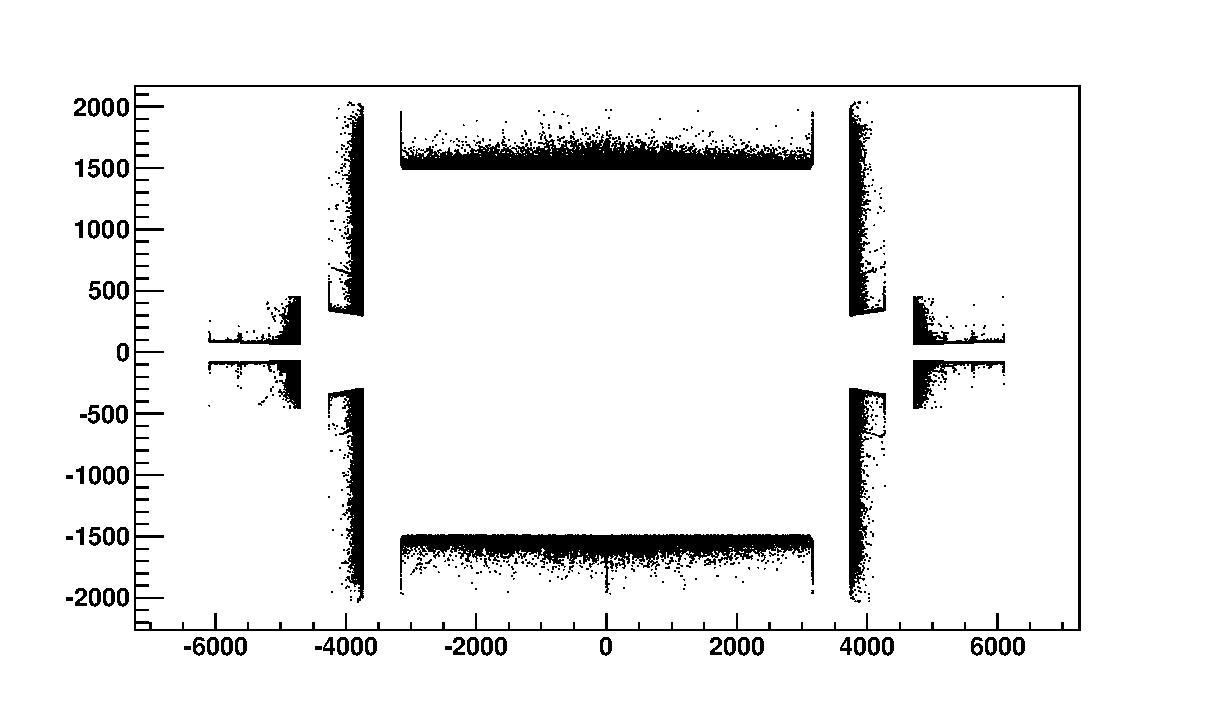
\includegraphics[width=1.0\textwidth]{figures/MC_FS_stpoints.eps}
\caption{The first stage of the 2-staged library production: FS starting point generation}
\label{fig:MC_FS_stpoints}}
\end{figure}

\begin{figure}
\center{
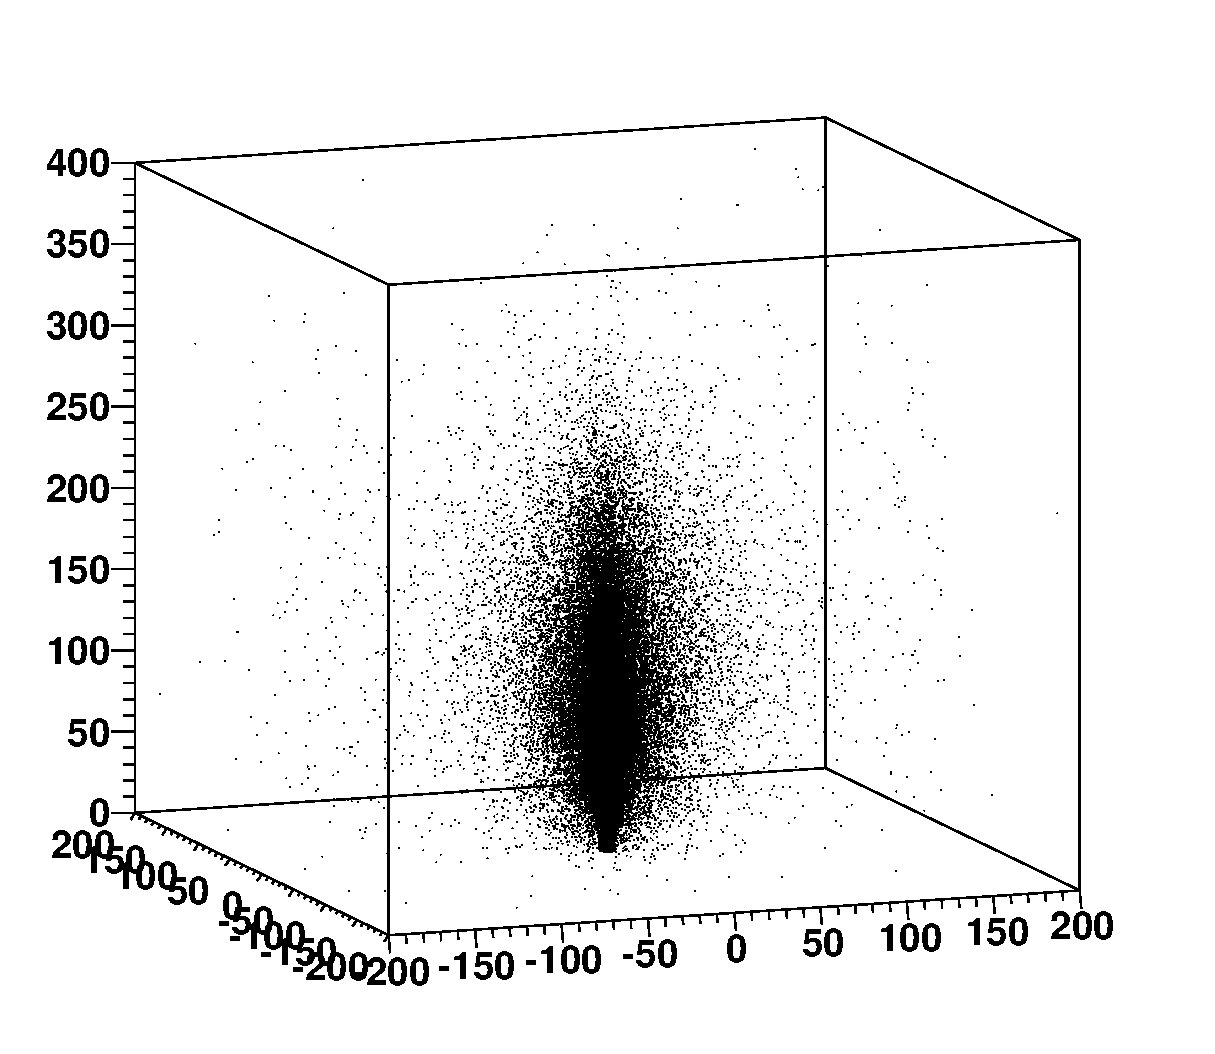
\includegraphics[width=0.75\textwidth]{figures/MC_FS_shower.eps}
\caption{The second stage of the 2-staged library production: the simulation of the shower}
\label{fig:MC_FS_shower}}
\end{figure}

This way of library generation solves all the problems mentioned above. The bin population problem does not occur because we produce the showers based on the physical MC samples, and the resulting size of each kinematic bin is in direct dependence of the number of times this bin is used. This allows to reduce the size of the library and yet make a bigger diversity.

The post-processing stage consists of merging of the adjacent hits and of removing the far-standing hits that won't contribute to the reconstructed cluster anyway. Also, during this stage the size of the shower is calculated. It is used for containment check during the production (which is when we check if the shower we are about to substitute the particle with is fully contained within the target detector).

The tuning of the library can then be applied manually in order to make the results the FS simulation closer to the standard simulation (also called "full simulation") or the data. As this is a process that can't be (as of yet) done automatically, it requires lots of time and effort.

\subsubsection{FS production use}
\label{sec:MC_FS_prod}

During the production run the simulation software checks constantly if any particle agree with the fast-simulation criteria, which is the energy range (should be low enough) and the sub-detector containment (the particle should be far enough from the edges of the sub-detector volume for shower to fit within). The containment check is energy-dependent, because the sizes of the showers grow with energy, and the more energetic particles should be further from the edges in order for shower to fit.

When the particle with the proper parameters is found, it is then removed from the simulation and replaced with the shower. Before the deposition, the shower is scaled to fully correspond to the particle in energy.

\begin{figure}
\center{
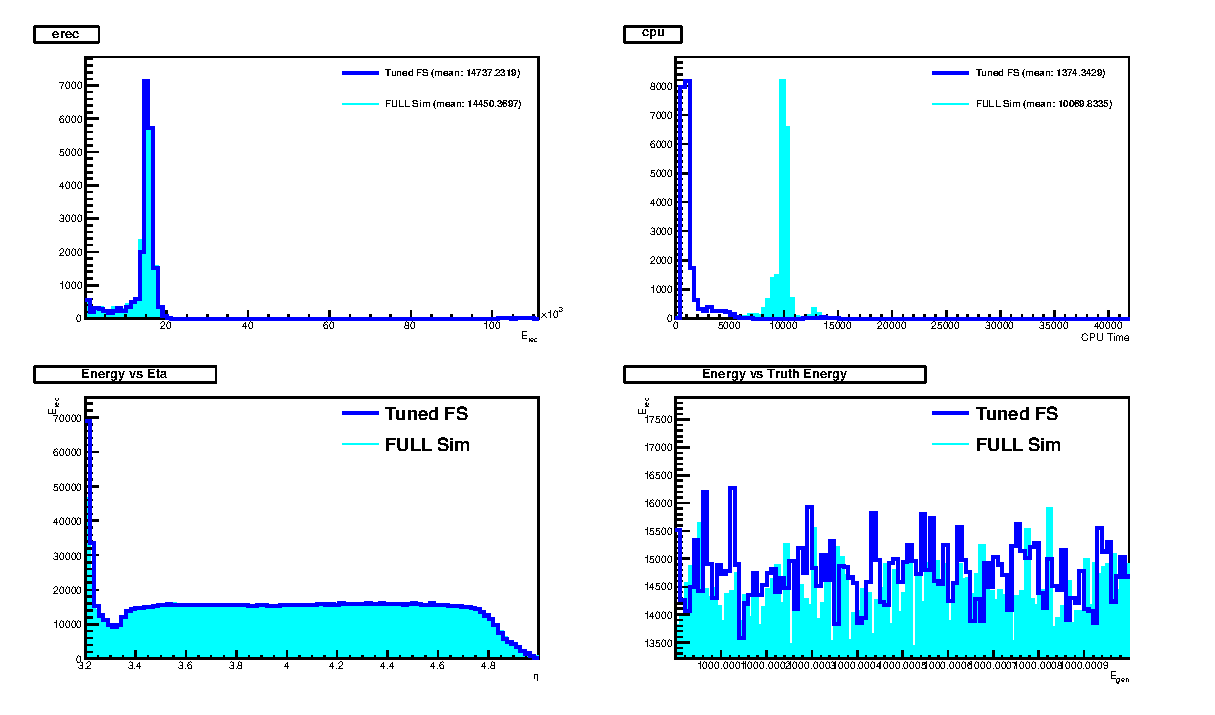
\includegraphics[width=1.0\textwidth]{figures/MC_FS_speedup.eps}
\caption{The simulation result for single electrons with energy 1000~GeV. CPU speed-up can be seen in top right. \tbu A BETTER PLOT}
\label{fig:MC_FS_speedup}}
\end{figure}

For the MC11c and MC11d campaigns, the data from which is used in this analysis, frozen showers system was enabled by default in FCAL. Several studies showed that the differences introduced by the FS is negligible compared to the differences between MC and data, while the simulation speedup was about 25\%. The smallness of the errors introduced by the FS compared to other fast simulation methods (most notably - FastCaloSim) leaded to the misunderstanding, when the simulation with the FS system enabled was called "full simulation" as opposed to other, less precise but faster methods, which were called "fast simulation". In this terminology, all of the MC samples used in this analysis are full simulations.

The sample comparison of the default, non-accelerated MC samples with the samples with enabled frozen showers can be seen in Fig.~\ref{fig:MC_FS_speedup}. It can be seen that the speed-up is significant, while the results remain the same.

\section{MC samples used in analysis}
\label{sec:MC_periods}

During this analysis the MC samples from both MC11c and MC11d campaigns were used. The "d" is chronologically the fourth sample produced for the 2011 data, and the "c" is the third. The decision to make new samples is usually made when some errors in GEANT software or in ATLAS geometry are discovered. The latest "d" sample fixes all such known errors, which affected the electron performance in various cases. The "d" is thus used in cases where the electron performance is important. The main generator used for both signal and background was \Powheg\ with the parton showering provided by \Pythia. The cross-check was done by the same \Powheg\ with the PS done by \Herwig\, and by \Mcatnlo\ also with the \Herwig-provided showers. For the
\Mcatnlo\ and \Powheg\ matrix element calculations the \pdfCteq\ PDF set is used, while showering was performed with \pdfCteql PDF. The list of MC signal periods that was used can be found in Tab.~\ref{tab:MC_periods}, the periods for MC background events are in Tab.~\ref{tab:MC_bg}.

\begin{table}
  \begin{center}
    \begin{tabular}{@{ } l @{ }| r @ { } | @{ } r @{ } | @{ }r@{}}
      \hline
      \hline
      Data set & Generator& $\sigma{\cdot}\text{BR}{\cdot}\epsilon_{filter}$ [nb] & $N_{evt}\,[10^6]$\\
      \hline

      108303$^{\mathrm{d}}$ &   \Powheg\Pythia & 1.006 (5\%) & 20\\

      126006 &   \Powheg \Herwig & 1.006 (5\%) & 10\\

      106087 \&~129913 & \Mcatnlo & 0.990 (5\%) & 5+5\\

      147770 & \Sherpa & 1.070 (5\%) & 10 \\

      \hline
    \end{tabular}
    \caption{Signal Monte Carlo samples. The sample marked with $^{\mathrm{d}}$ was taken from the MC11d campaign, the others are from the MC11c.}
    \label{tab:MC_periods}
  \end{center}
\end{table}

\begin{table}
  \begin{center}
    \begin{tabular}{@{} l @ { }|@{ } l @{ }| r @ { } | @{ } r @{ } | @{ }r@{}}
      \hline
      \hline
      Process & Data set & Generator & $\sigma{\cdot}\text{BR}{\cdot}\epsilon_{filter}$ [nb] & $N_{evt}\,[10^6]$\\
      \hline

      \Wplusenu       & 108297$^{\mathrm{d}}$  &  \Powheg\Pythia  &
      6.160 (5\%) & 23 \\
      \Wminusenu & 108300$^{\mathrm{d}}$  &  \Powheg\Pythia &
      4.300 (5\%) & 17 \\
      \Wplusenu       & 113186 &  \Powheg\Herwig  &
      6.160 (5\%) & 16 \\
      \Wminusenu & 113184 &  \Powheg\Herwig &
      4.300 (5\%) & 12 \\
      \Wplusenu       & 106080 & \Mcatnlo &
      6.160 (5\%) & 16 \\
      \Wminusenu & 106081 & \Mcatnlo &
      4.300 (5\%) & 12 \\

      \hline

      \Wtau\ Np0   &  107700 &  \Alpgen\Herwig\ & 8.285 (5\%) & 3.4 \\
      \Wtau\ Np1   &  107701 &  \Alpgen\Herwig\ & 1.560 (5\%) & 2.5 \\
      \Wtau\ Np2   &  107702 &  \Alpgen\Herwig\ & 0.452 (5\%) & 3.8 \\
      \Wtau\ Np3   &  107703 &  \Alpgen\Herwig\ & 0.122 (5\%) & 1 \\
      \Wtau\ Np4   &  107704 &  \Alpgen\Herwig\ & 0.0307 (5\%) & 0.25 \\
      \Wtau\ Np5   &  107705 &  \Alpgen\Herwig\ & 0.00835 (5\%) & 0.07 \\
      \Wtau        &  107054 &  \Pythia\        & 10.460 (5\%) & 1 \\
      \Wplusenu & 147412$^{\mathrm{d}}$  &  \Powheg\Pythiaeight  &
      6.160 $\cdot$ 0.1510 (5\%) & 15 \\
      \Wminusenu & 147415$^{\mathrm{d}}$  &  \Powheg\Pythiaeight  &
      4.300 $\cdot$ 0.1404 (5\%) & 10 \\
      \hline

      \Ztau\ Np0  &  107670 &  \Alpgen\Herwig\  & 0.834 (5\%) & 6.6 \\
      \Ztau\ Np1  &  107671 &  \Alpgen\Herwig\  & 0.168 (5\%) & 1.3 \\
      \Ztau\ Np2  &  107672 &  \Alpgen\Herwig\  & 0.0508 (5\%) & 0.81 \\
      \Ztau\ Np3  &  107673 &  \Alpgen\Herwig\  & 0.0140 (5\%) & 0.22 \\
      \Ztau\ Np4  &  107674 &  \Alpgen\Herwig\  & 0.00355 (5\%) & 0.06 \\
      \Ztau\ Np5  &  107675 &  \Alpgen\Herwig\  & 0.00093 (5\%) & 0.02 \\
      \Ztau\      &  106052 &  \Pythia\         & 0.990 (5\%) & 3\\
      \Ztau & 147418$^{\mathrm{d}}$ &   \Powheg\Pythiaeight   &
      0.990 $\cdot$ 0.263 (5\%) & 6\\
      \hline

      \ggee & 129652 & \Pythiaeight & $2.41\cdot 10^{-3} \cdot 0.7$ (40\%) & 0.5\\

      \hline

      \ttbar  & 105200$^{\mathrm{d}}$ & \Mcatnlo & $0.1773\, (6.2\%) \cdot \, 0.555$ & 1.5\\

      \hline

      $WW$ & 105985$^{\mathrm{d}}$ & \Herwig & 44.9 $\cdot$ 0.389 $\cdot 10^{-3}$ (7\%) & 1.5 \\
      $WZ$ & 105987$^{\mathrm{d}}$ & \Herwig & 18.5 $\cdot$ 0.310 $\cdot 10^{-3}$ (7\%) & 1 \\
      $ZZ$ & 105986$^{\mathrm{d}}$ & \Herwig & 6.02 $\cdot$ 0.212 $\cdot 10^{-3}$ (7\%) &
      0.25 \\

      \hline
    \end{tabular}
    \caption{ Background Monte Carlo samples. The samples marked with $^{\mathrm{d}}$ were taken from the MC11d campaign, the others are from the MC11c. }
    \label{tab:MC_bg}
  \end{center}
\end{table}

\section{Reweightings}
\label{sec:MC_correction}

The MC samples have a number of known shortcomings, and some data distributions are not described well. To fix this we apply reweightings based on MC/data comparisons at the reconstruction levels, different MCs comparisons on the generation (truth) level, or using the other ATLAS analyses. The weights are applied based on the truth information and are validated using the closure tests. The list of corrections is this:

\begin{itemize}
\item \textbf{Pileup Reweighting} is based on the $\mu$ variable and aims to equalize the amount of pileup in MC and data. This is done using the \texttt{PileupReweighting} tool~\cite{lib:pileuptool, lib:pileupscale}. The difference between data and MC in pileup conditions can be seen in Fig.~\ref{fig:MC_pileup}.
\item \textbf{Vertex Spread in $z$ Reweighting} is based on the $z$ component of the vertex and aims to decrease the spread of the beam spot in $z$-direction of MC, which is significantly smaller in data (for data $\sigma_z \approx 56$mm, while for narrow beam spot MC sample $\sigma_z = 75$mm and for wide beam spot $\sigma_z = 90$mm). The \texttt{VertexPositionReweightTool} is used for that. The effect of this correction can be seen in Fig.~\ref{fig:MC_zvtx}.
\item \textbf{$Z$ Boson $p_T$ Reweighting} is applied to the $p_T$ distribution of the $Z$ bosons, which doesn't describe the data well in the MC signal generators used for this analysis. The results from ATLAS $Z$ $\phi^*$ and $\pt$ analyses~\cite{lib:Zphistar} were used for it, and it was done using the \texttt{BosonPtReweightingTool}.
\item \textbf{$Z$ Boson Line Shape Reweighting} is the reweightings aimed to fix the fundamental shortcomings of the MC generators caused by the electroweak order not being high enough. This reweighting is done using the \texttt{LineShapeTool}. See~\cite{lib:lineshape} for details.
\end{itemize}

\begin{figure}
\center{
\subfigure[$z_{vtx}$ weights] {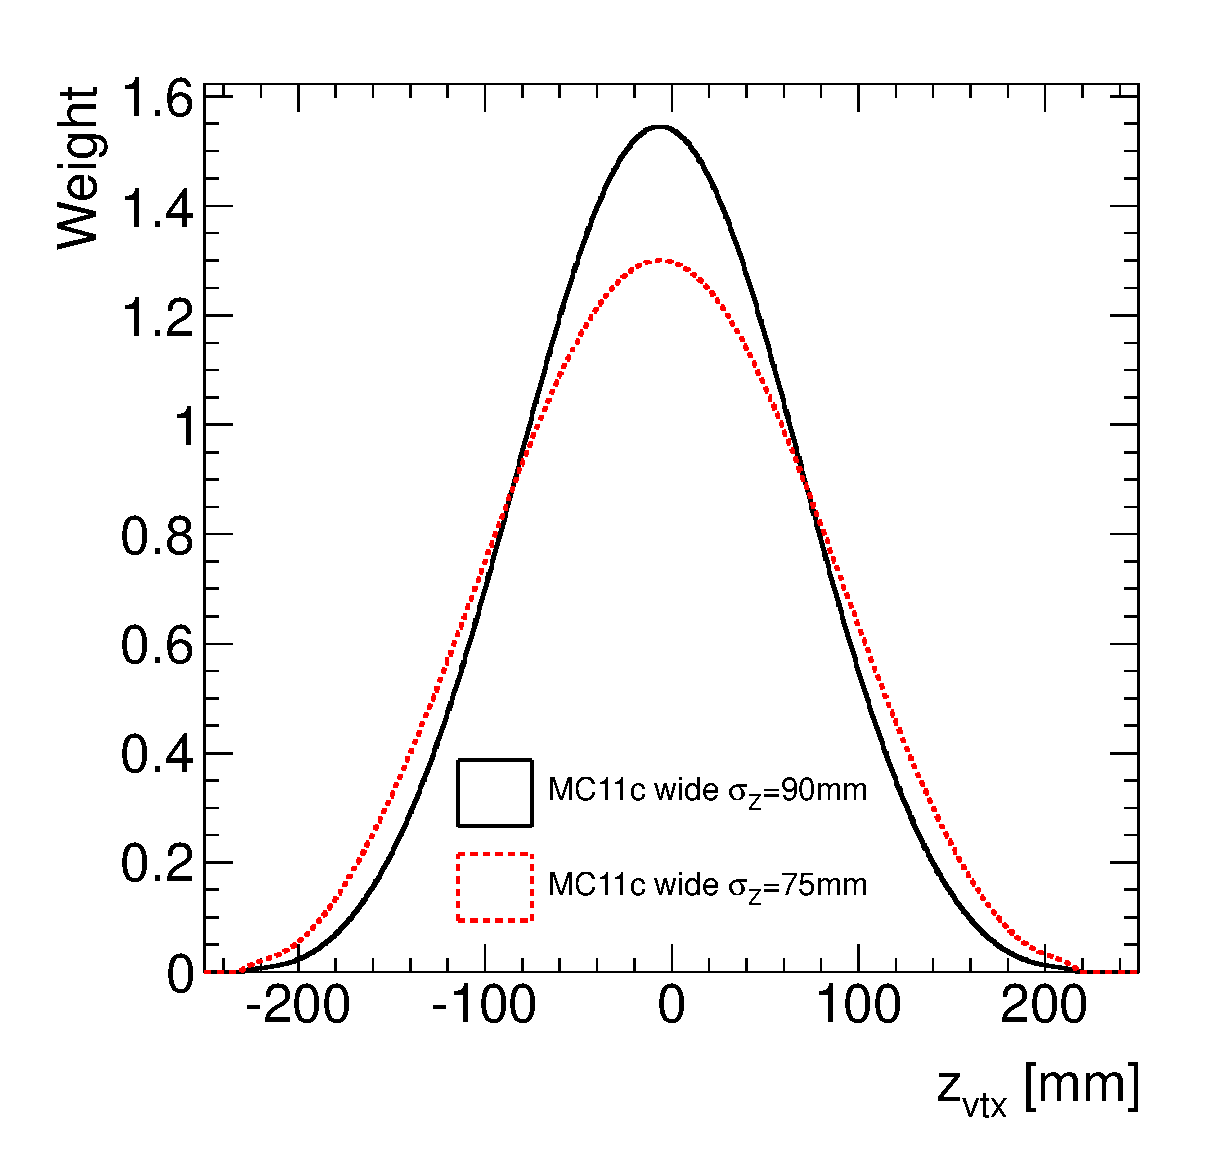
\includegraphics[width=0.32\textwidth]{figures/MCrew_zvtx_weights.eps}}
\subfigure[Before $z_{vtx}$ reweight] {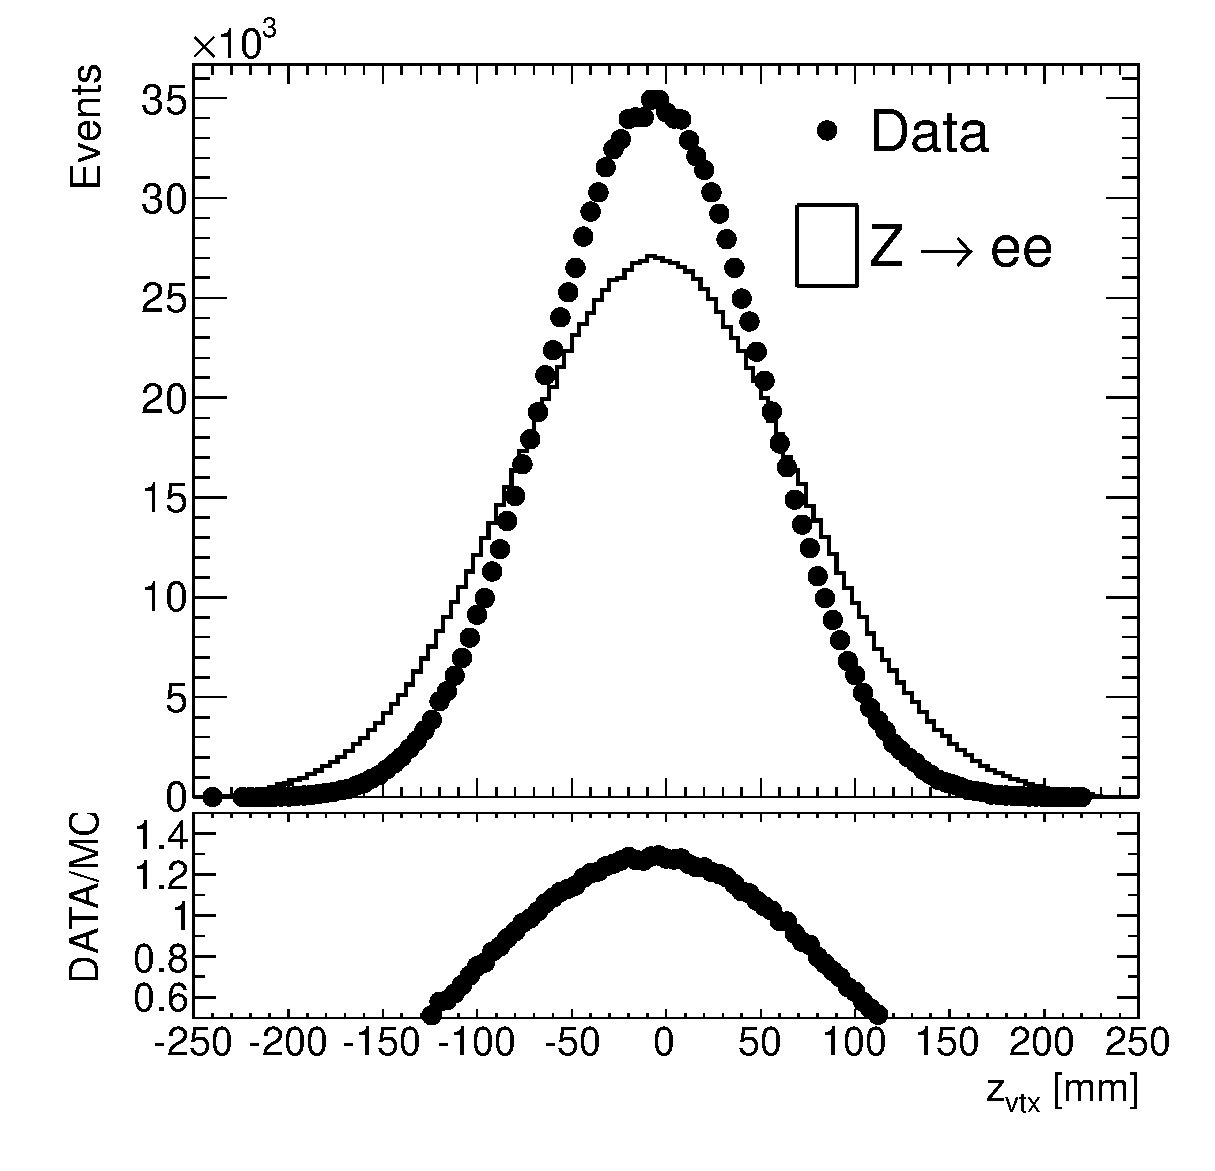
\includegraphics[width=0.32\textwidth]{figures/MCrew_zvtx_before.eps}}
\subfigure[After $z_{vtx}$ reweight] {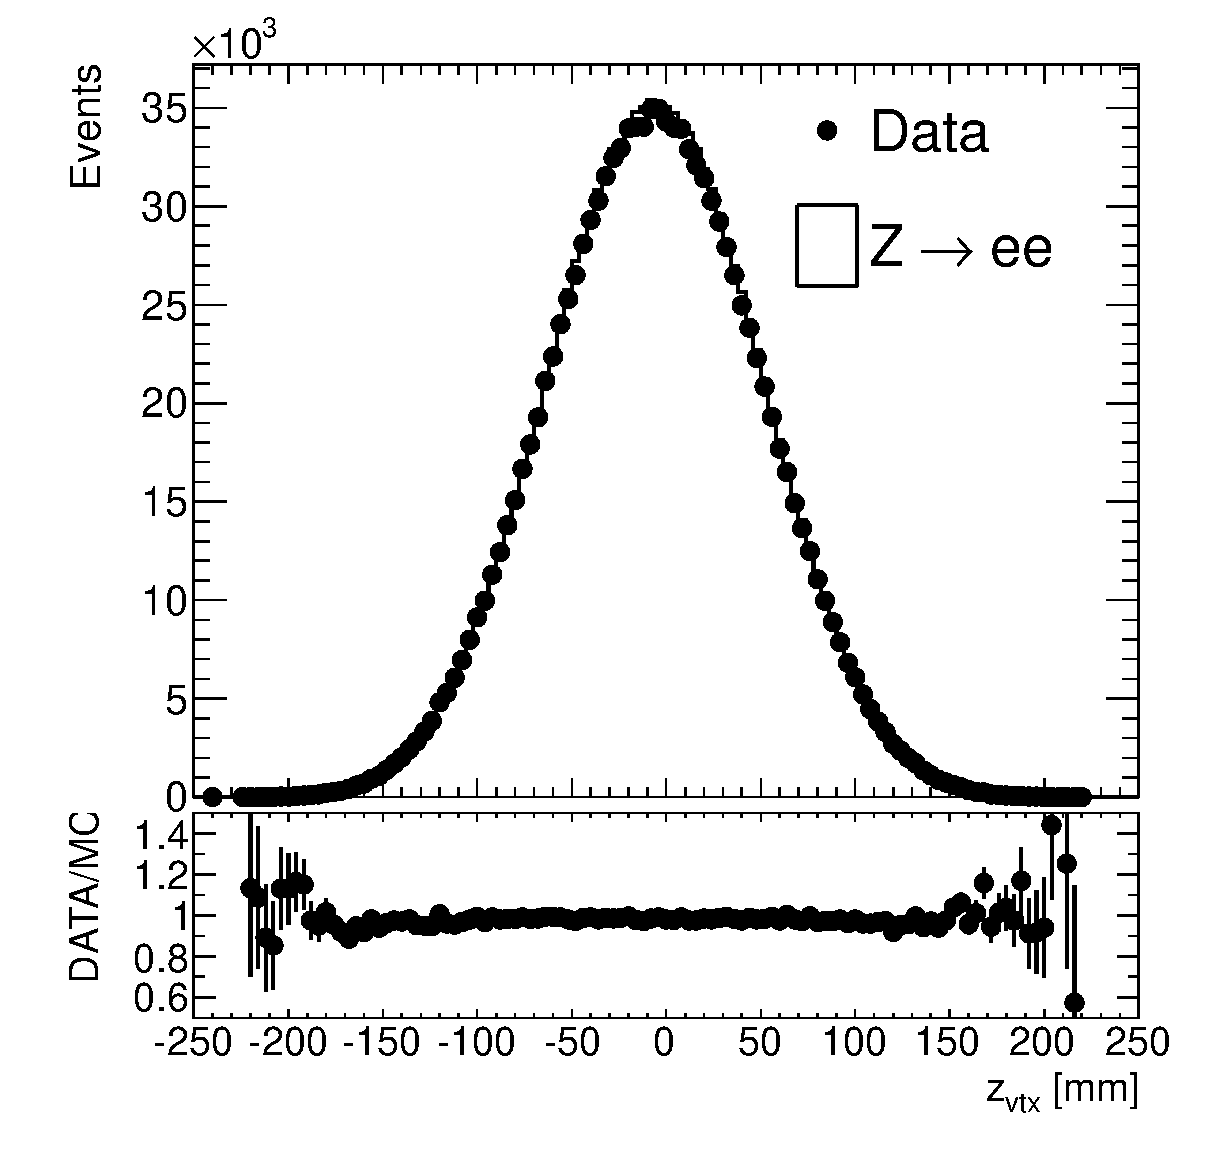
\includegraphics[width=0.32\textwidth]{figures/MCrew_zvtx_after.eps}}
\caption{The effect of the vertex spread correction applied to MC11c samples. The corrections for MC11d remained the same.}
\label{fig:MC_zvtx}}
\end{figure}

\begin{figure}
\center{
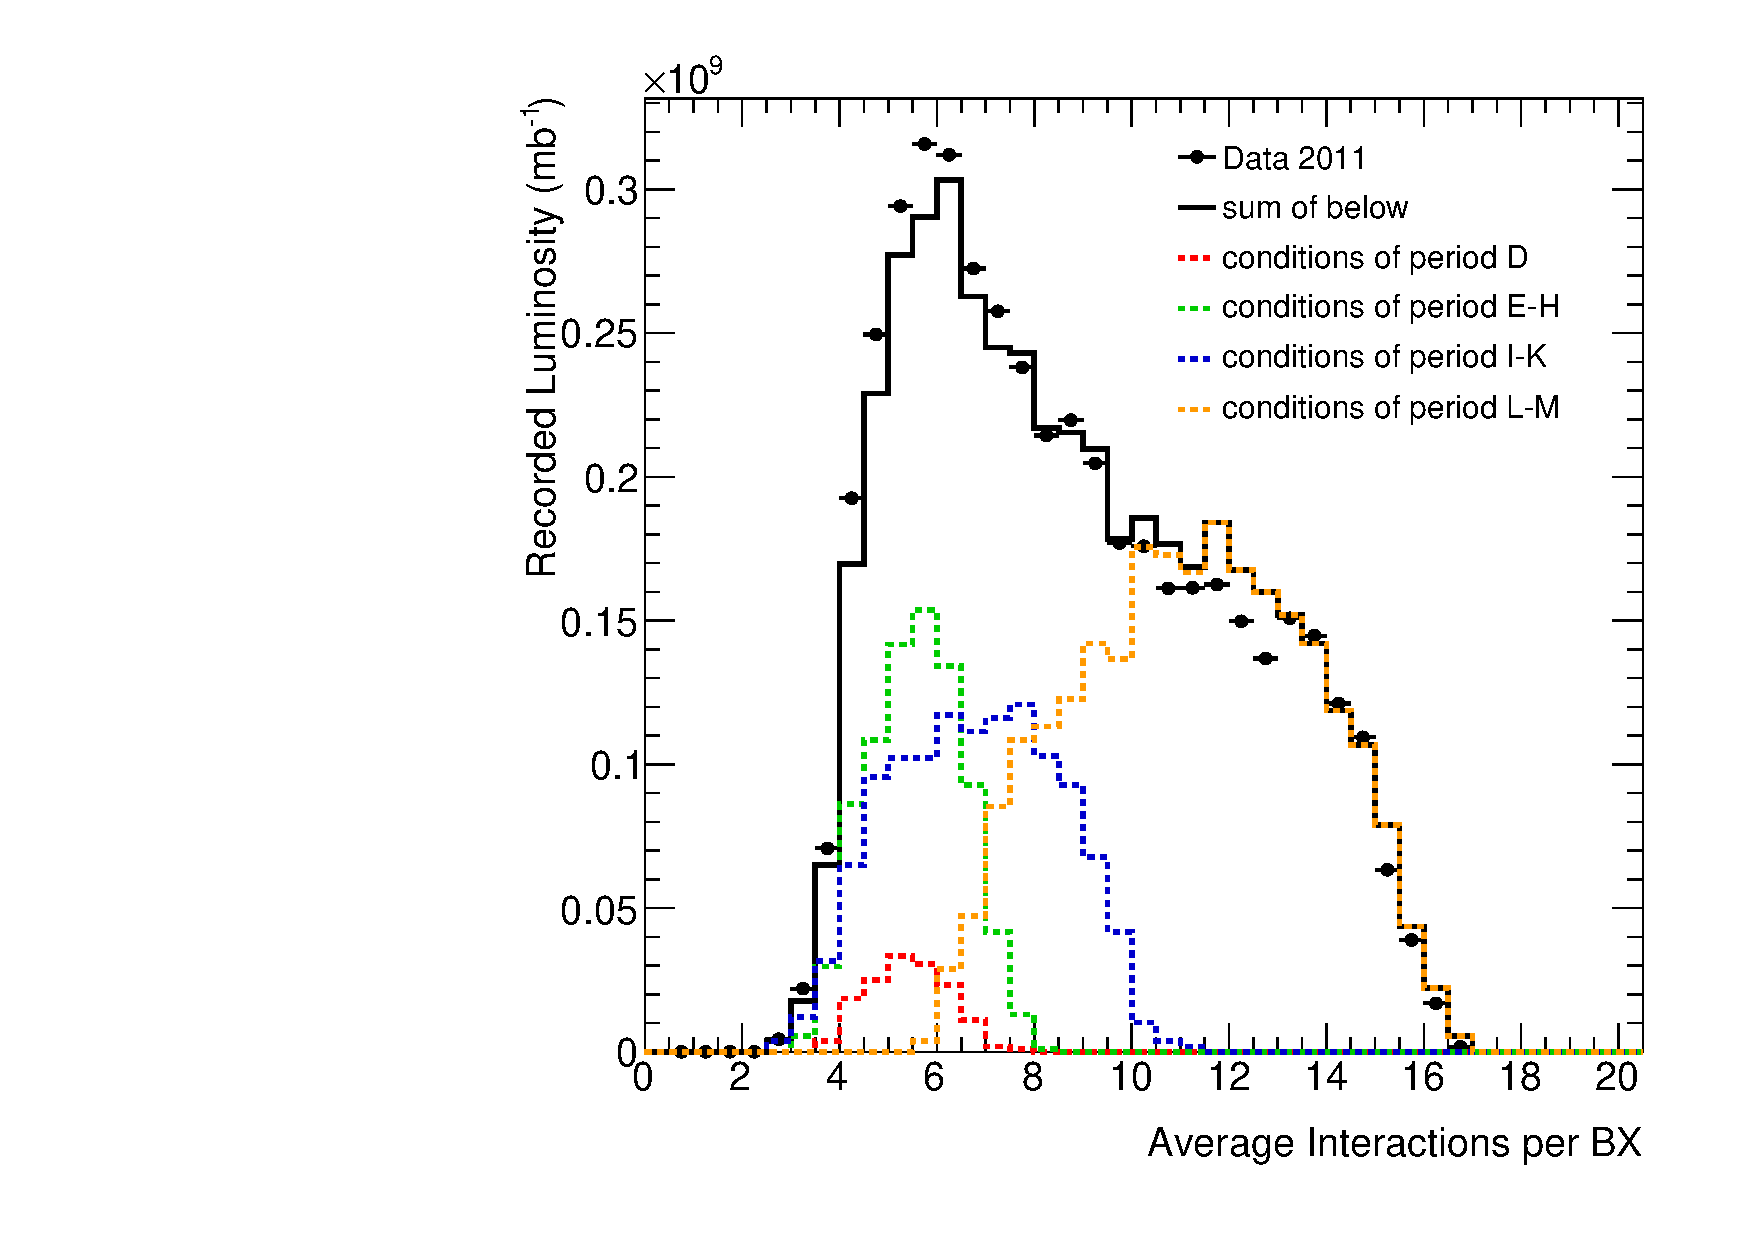
\includegraphics[width=0.6\textwidth]{figures/MCrew_pileup.pdf}
\caption{The comparison of the pileup conditions of the MC11c and 2011 data. The pileup conditions for different MC periods is also shown.}
\label{fig:MC_pileup}}
\end{figure}
